\section{Analisi dei Requisiti}
\textit{Dal 2020-12-13 al 2021-01-18}


\begin{figure}[H]
	\centering
	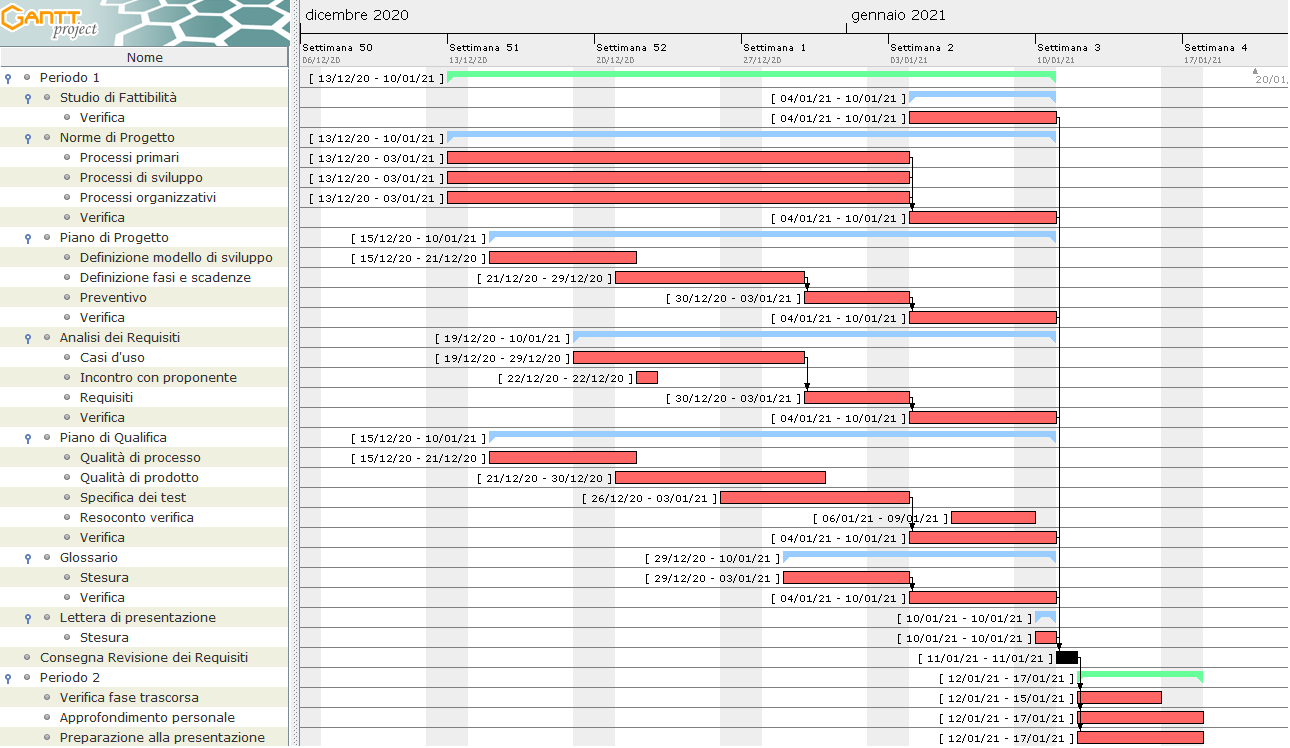
\includegraphics[scale=0.43]{res/images/gantt_fase/02_gantt_analisi_requisiti.png}
	\caption{Diagramma di Gantt\textsubscript{G} relativo all'Analisi dei Requisiti}
\end{figure}


\subsection{Periodo 1}

\subsubsection{Pianificazione preventiva}

\paragraph{Attività}
\subparagraph*{}

\planningTable{
	Studio di Fattibilità & Si verifica lo \textsc{Studio di Fattibilità} redatto durante la fase\textsubscript{G} di Avvio & 2 & Verificatore
\tabularnewline 
Norme di Progetto & Vengono stabilite le norme di progetto\textsubscript{G} pianificando nel dettaglio i processi primari, i processi di sviluppo e i processi organizzativi. Il documento \textsc{Norme di Progetto} viene redatto & 22 & Amministratore
\tabularnewline 
Piano di Progetto & Il Responsabile di Progetto redige il \textsc{Piano di Progetto} scandendo le fase\textsubscript{G} e i periodi secondo cui si articolerà il lavoro & 20 & Responsabile
\tabularnewline 
Analisi dei Requisiti & Uno studio approfondito del capitolato\textsubscript{G} e ne individuano i requisiti\textsubscript{G}: l'analisi si caratterizza da contatti frequenti con il proponente che fornirà supporto nella comprensione del problema. Viene completata la redazione dell'\textsc{Analisi dei Requisiti} & 50 & Analista
\tabularnewline 
Piano di Qualifica & In questa attivita\textsubscript{G} si individuano i criteri che garantiscono la qualità del prodotto. Viene redatto il \textsc{Piano di Qualifica} & 20 & Verificatore
\tabularnewline 
Glossario & Il \textsc{Glossario} conterrà i termini a cui si riterrà necessario dare definizione & 3 & Responsabile
\tabularnewline 
Verifica dei documenti & Quest'attività si concentra nella settimana che precede la presentazione e ha l'obiettivo di verificare e certificare la qualità di tutti i documenti prodotti & 23 & Verificatore
\tabularnewline 
Lettera di Presentazione & Avviene la stesura della lettera con cui il gruppo si candida alla Revisione dei Requisiti & 1 & Responsabile
\tabularnewline 
\caption{Pianificazione preventiva - Analisi dei Requisiti - Periodo 1}
}


\paragraph{Preventivo}
\subparagraph*{}

\hspace{-1cm}
\begin{minipage}{.50\textwidth}
\smallPreventivoTable{
	Responsabile & 24 & 720\\ 
Verificatore & 45 & 675\\ 
Analista & 50 & 1250\\ 
Amministratore & 22 & 440\\ 
Programmatore & 0 & 0\\ 
Progettista & 0 & 0\\ 
\hlinetable 
\textbf{Totale} & \textbf{141} & \textbf{3085}\\ 
\end{tabular} 
\caption{Preventivo - Analisi dei Requisiti - Periodo 1}
}
\end{minipage}
\hspace{1cm}
\begin{minipage}{.40\textwidth}
\begin{figure}[H]
	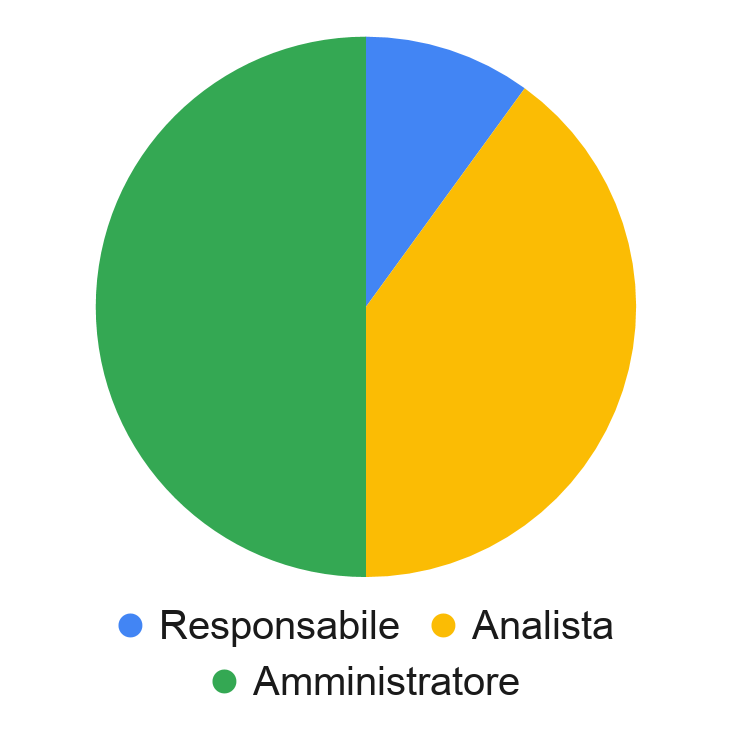
\includegraphics[scale=0.21]{res/images/charts/preventivo_priori/Grafico4-1.png}
	\caption{Distribuzione dei costi: preventivo - Analisi dei Requisiti - Periodo 1}
\end{figure}\end{minipage} 


\subsubsection{Pianificazione di periodo}

\paragraph{Preventivo orario ed economico}
\subparagraph*{}

\contabilitaTable{
	Chiarello Sofia & 0 & 6 & 16 & 1 & 0 & 0 & \textbf{23}\\ 
Crivellari Alberto & 0 & 18 & 4 & 2 & 0 & 0 & \textbf{24}\\ 
De Renzis Simone & 11 & 5 & 5 & 3 & 0 & 0 & \textbf{24}\\ 
Greggio Nicolò & 5 & 5 & 5 & 9 & 0 & 0 & \textbf{24}\\ 
Tessari Andrea & 8 & 5 & 4 & 6 & 0 & 0 & \textbf{23}\\ 
Zuccolo Giada & 0 & 6 & 16 & 1 & 0 & 0 & \textbf{23}\\ 
\hlinetable 
\textbf{Totale orario} & \textbf{24} & \textbf{45} & \textbf{50} & \textbf{22} & \textbf{0} & \textbf{0} & \textbf{141}\\ 
\textbf{Totale costo} & \textbf{720} & \textbf{675} & \textbf{1250} & \textbf{440} & \textbf{0} & \textbf{0} & \textbf{3085}\\ 
\end{tabular} 
\caption{Preventivo di periodo\textsubscript{G} - Analisi dei Requisiti - Periodo 1}
}

\begin{figure}[H]
	\centering
	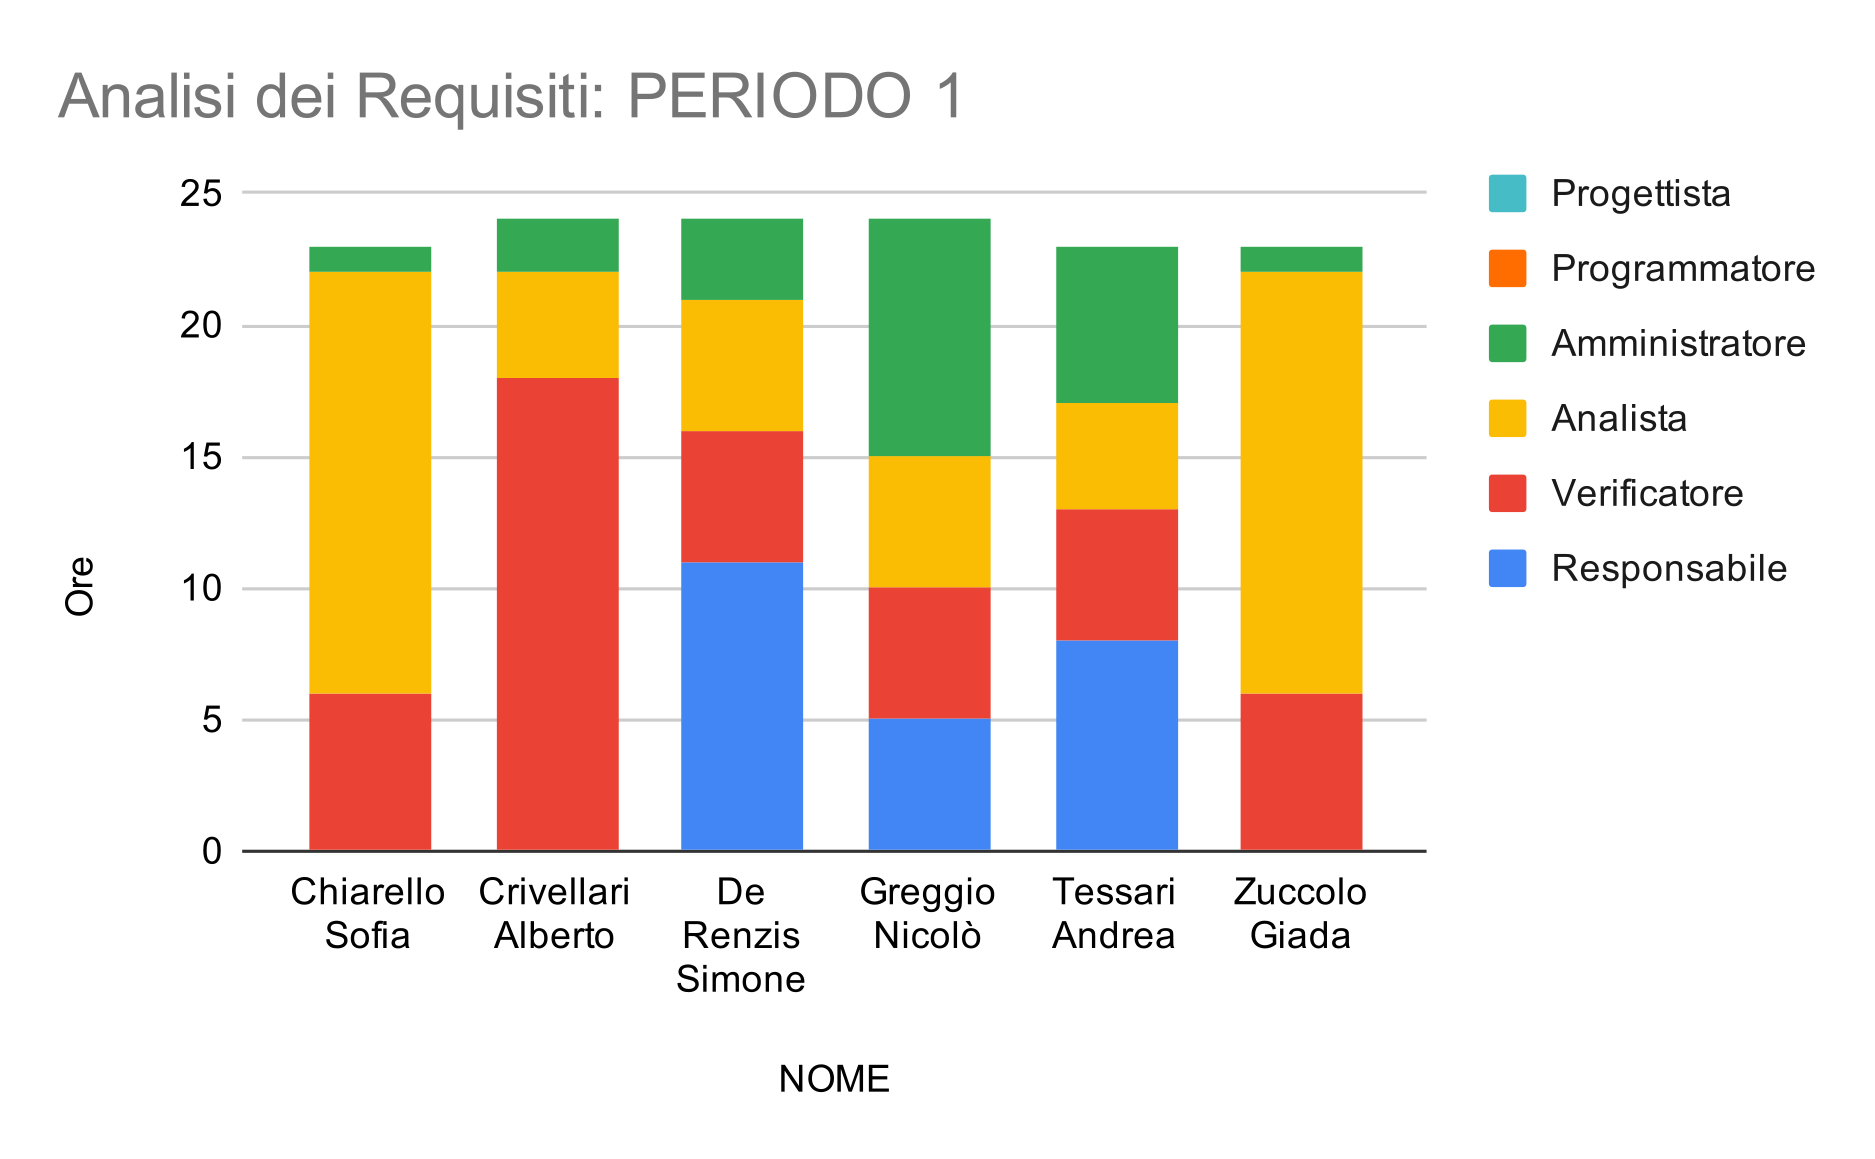
\includegraphics[scale=2]{res/images/charts/preventivo/analisi_1.png}
	\caption{Distribuzione oraria per componente: preventivo di periodo\textsubscript{G} - Analisi dei Requisiti - Periodo 1}
\end{figure}


\subsubsection{Riscontro di fine periodo}


\paragraph{Consuntivo orario ed economico}
\subparagraph*{}

\contabilitaTable{
	Chiarello Sofia & 3 & 4 & 14 & 3 & 0 & 0 & \textbf{24} \\ 
Crivellari Alberto & 4 & 11 & 4 & 5 & 0 & 0 & \textbf{24} \\ 
De Renzis Simone & 10 & 4 & 5 & 4 & 0 & 0 & \textbf{23} \\ 
Greggio Nicolò & 4 & 2 & 5 & 22 & 0 & 0 & \textbf{33} \\ 
Tessari Andrea & 8 & 9 & 4 & 2 & 0 & 0 & \textbf{23} \\ 
Zuccolo Giada & 3 & 6 & 12 & 3 & 0 & 0 & \textbf{24} \\ 
\hlinetable 
\textbf{Totale orario} & \textbf{32} & \textbf{36} & \textbf{44} & \textbf{39} & \textbf{0} & \textbf{0} & \textbf{151} \\ 
\textbf{Differenza orario} & \textbf{8} & \textbf{-9} & \textbf{-6} & \textbf{17} & \textbf{0} & \textbf{0} & \textbf{10} \\ 
\textbf{Totale costi} & \textbf{960} & \textbf{540} & \textbf{1100} & \textbf{780} & \textbf{0} & \textbf{0} & \textbf{3380} \\ 
\textbf{Differenza costi} & \textbf{240} & \textbf{-135} & \textbf{-150} & \textbf{340} & \textbf{0} & \textbf{0} & \textbf{295} \\ 
\end{tabular} 
\caption{Consuntivo - Analisi dei Requisiti - Periodo 1}
}

\begin{figure}[H]
	\centering
	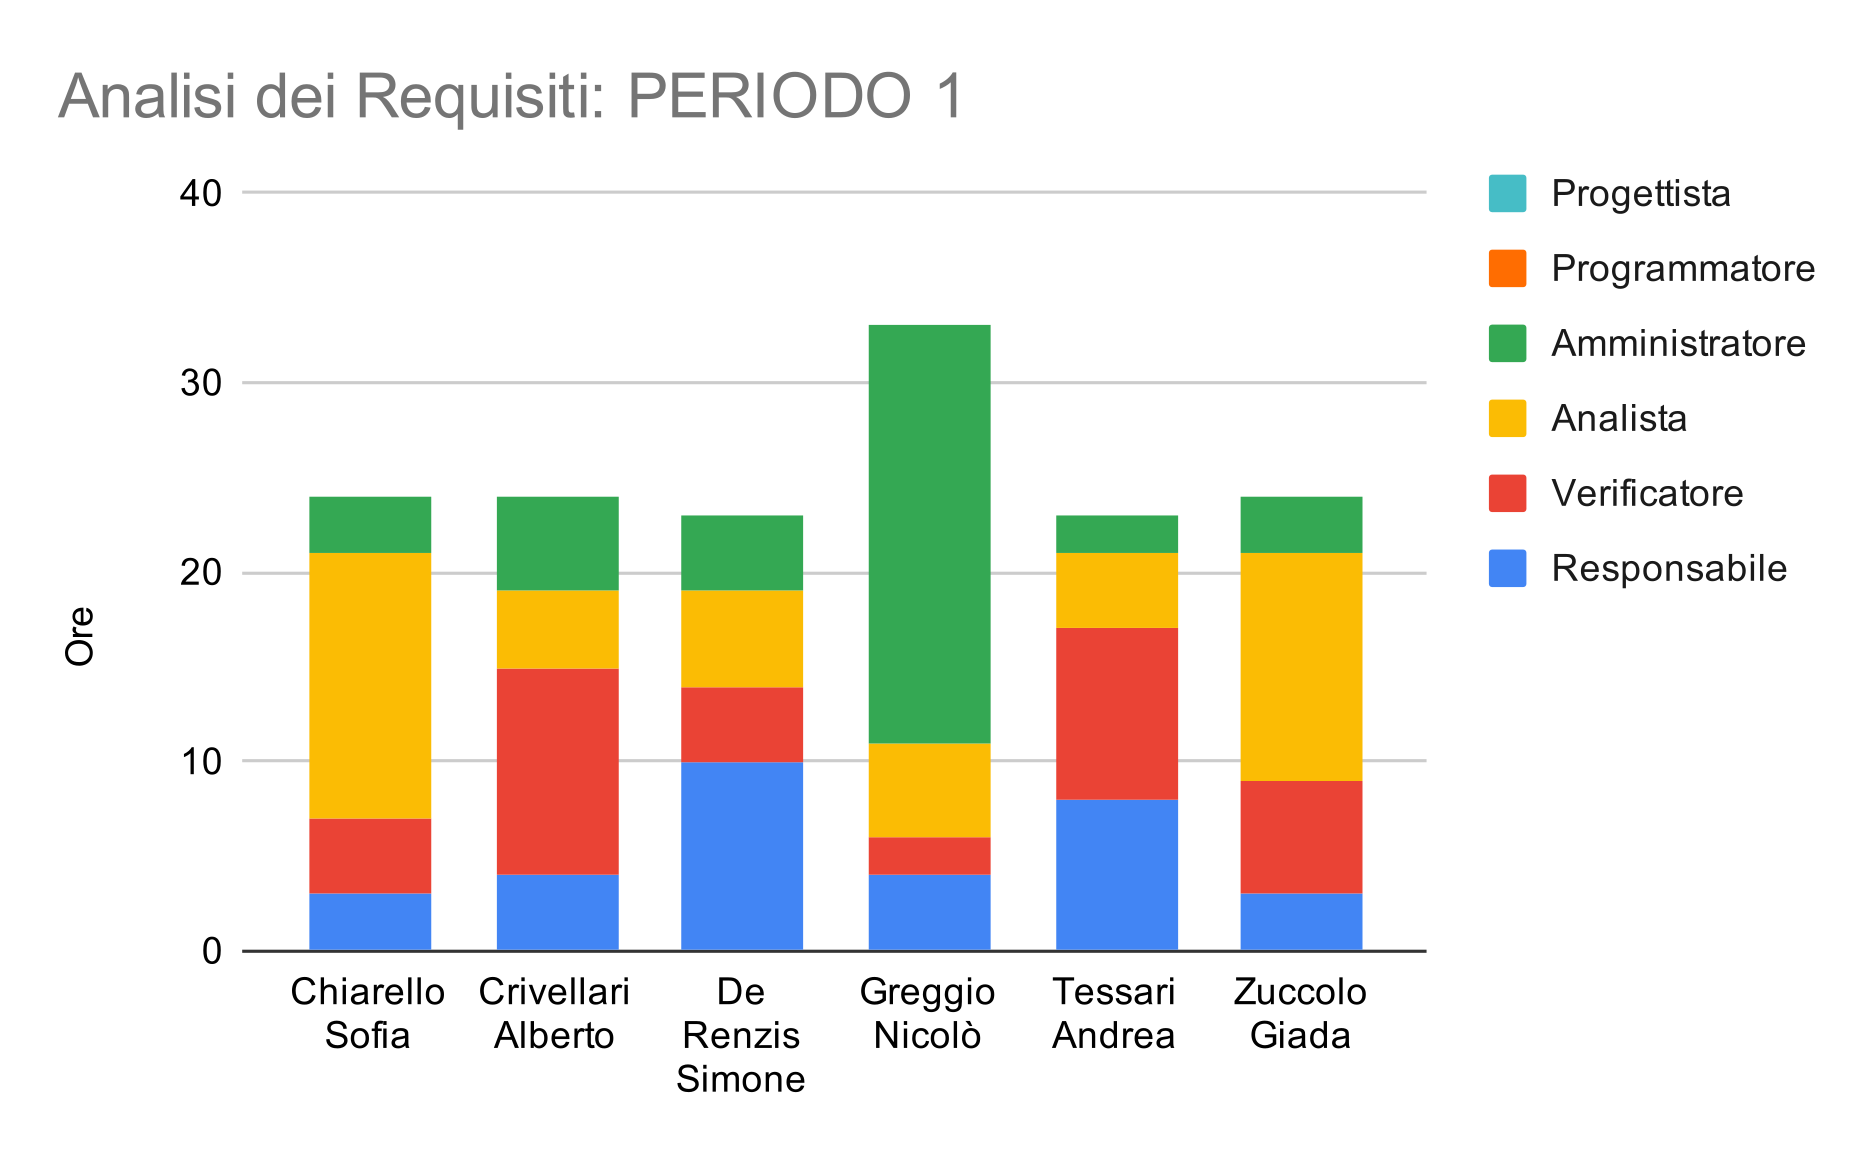
\includegraphics[scale=2]{res/images/charts/consuntivo/analisi_1.png}
	\caption{Distribuzione oraria per componente: consuntivo - Analisi dei Requisiti - Periodo 1}
\end{figure}

Il periodo\textsubscript{G} chiude in \textbf{negativo}, costringendo il gruppo ad una spesa supplementare di \textbf{295 \euro}. I ruoli di Responsabile e Amministratore hanno richiesto più tempo di quando preventivato: gli sforzi di pianificazione e organizzazione degli strumenti di lavoro si sono rivelati impegnativi e dispendiosi. \'E stato probabilmente necessario svolgere attività\textsubscript{G} che sarebbero state meglio collocate nell'Avvio.



\paragraph{Preventivo a finire}
\subparagraph*{}

\pafTable{
	Avvio & 1 & Consuntivo & 1060
\tabularnewline
Analisi dei Requisiti & 1 & Consuntivo & 3380
\tabularnewline
Analisi dei Requisiti & 2 & Preventivo & 230
\tabularnewline
Progettazione Architetturale & 1 & Preventivo & 680
\tabularnewline
Progettazione Architetturale & 2 & Preventivo & 2414
\tabularnewline
Progettazione Architetturale & 3 & Preventivo & 280
\tabularnewline
Progettazione di Dettaglio e Codifica & 1 & Preventivo & 1270
\tabularnewline
Progettazione di Dettaglio e Codifica & 2 & Preventivo & 4097
\tabularnewline
Progettazione di Dettaglio e Codifica & 3 & Preventivo & 258
\tabularnewline
Validazione e Collaudo & 1 & Preventivo & 220
\tabularnewline
Validazione e Collaudo & 2 & Preventivo & 2145
\tabularnewline
Validazione e Collaudo & 3 & Preventivo & 60
\tabularnewline
\textbf{Totale} & \textbf{} & \textbf{} & \textbf{16094}
\tabularnewline
\textbf{Totale rendicontato} & \textbf{} & \textbf{} & \textbf{11424}
\tabularnewline
\caption{Preventivo a finire - Analisi dei Requisiti - Periodo 1}
}

\pagebreak
\subsection{Periodo 2}

\subsubsection{Pianificazione preventiva}

\paragraph{Attività}
\subparagraph*{}

\planningTable{
	Preparazione alla presentazione & Viene preparato il materiale necessario alla presentazione. & 5 & Amministratore
\tabularnewline 
Verifica dei macro periodi precedenti & Il gruppo si vede coinvolto in un confronto dal quale vorranno emergere le criticità riscontrate nel macro periodo\textsubscript{G} trascorso, al fine di migliorare lo svolgimento dei periodi successivi. & 1 & Responsabile
\tabularnewline 
Approfondimento personale & Ogni membro del gruppo spende alcune ore per formare e consolidare una conoscenza di base degli strumenti e tecniche da impiegare nel periodo\textsubscript{G} successivo. & 4 & Analista
\tabularnewline 
\caption{Pianificazione preventiva - Analisi dei Requisiti - Periodo 1}
}



\paragraph{Preventivo}
\subparagraph*{}

\hspace{-1cm}
\begin{minipage}{.50\textwidth}
\smallPreventivoTable{
	Responsabile & 1 & 30\\ 
Verificatore & 0 & 0\\ 
Analista & 4 & 100\\ 
Amministratore & 5 & 100\\ 
Programmatore & 0 & 0\\ 
Progettista & 0 & 0\\ 
\hlinetable 
\textbf{Totale} & \textbf{10} & \textbf{230}\\ 
\end{tabular} 
\caption{Preventivo - Analisi dei Requisiti - Periodo 1}
}
\end{minipage}
\hspace{1cm}
\begin{minipage}{.40\textwidth}
\begin{figure}[H]
	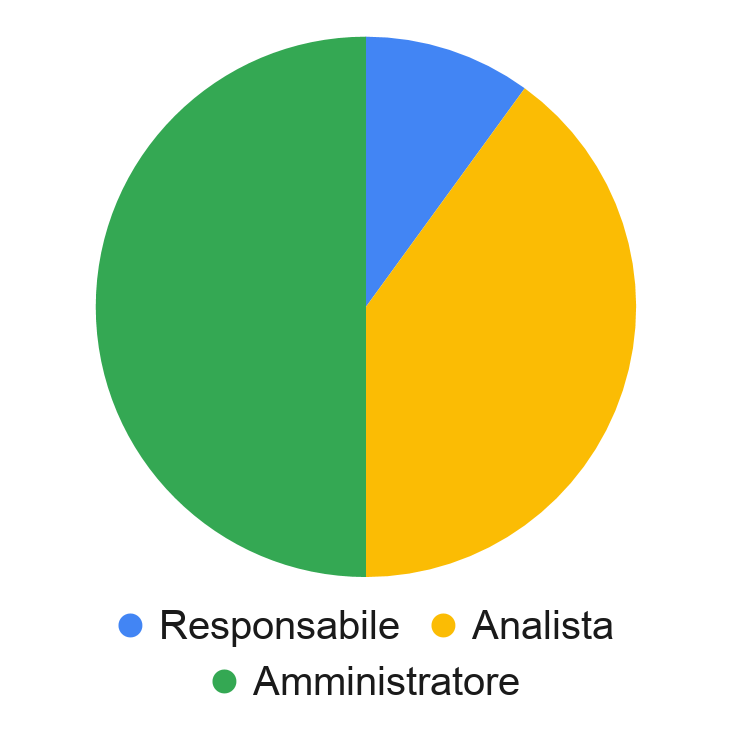
\includegraphics[scale=0.21]{res/images/charts/preventivo_priori/Grafico4-2.png}
	\caption{Distribuzione dei costi: preventivo - Analisi dei Requisiti - Periodo 2}
\end{figure}
\end{minipage} 


\subsubsection{Pianificazione di periodo}

\paragraph{Preventivo orario ed economico}
\subparagraph*{}

\contabilitaTable{
	Chiarello Sofia & 0 & 0 & 2 & 0 & 0 & 0 & \textbf{2}\\ 
Crivellari Alberto & 0 & 0 & 1 & 0 & 0 & 0 & \textbf{1}\\ 
De Renzis Simone & 1 & 0 & 0 & 1 & 0 & 0 & \textbf{2}\\ 
Greggio Nicolò & 0 & 0 & 0 & 2 & 0 & 0 & \textbf{2}\\ 
Tessari Andrea & 0 & 0 & 0 & 2 & 0 & 0 & \textbf{2}\\ 
Zuccolo Giada & 0 & 0 & 1 & 0 & 0 & 0 & \textbf{1}\\ 
\hlinetable 
\textbf{Totale orario} & \textbf{1} & \textbf{0} & \textbf{4} & \textbf{5} & \textbf{0} & \textbf{0} & \textbf{10}\\ 
\textbf{Totale costo} & \textbf{30} & \textbf{0} & \textbf{100} & \textbf{100} & \textbf{0} & \textbf{0} & \textbf{230}\\ 
\end{tabular} 
\caption{Preventivo di periodo\textsubscript{G} - Analisi dei Requisiti - Periodo 2}
}

\begin{figure}[H]
	\centering
	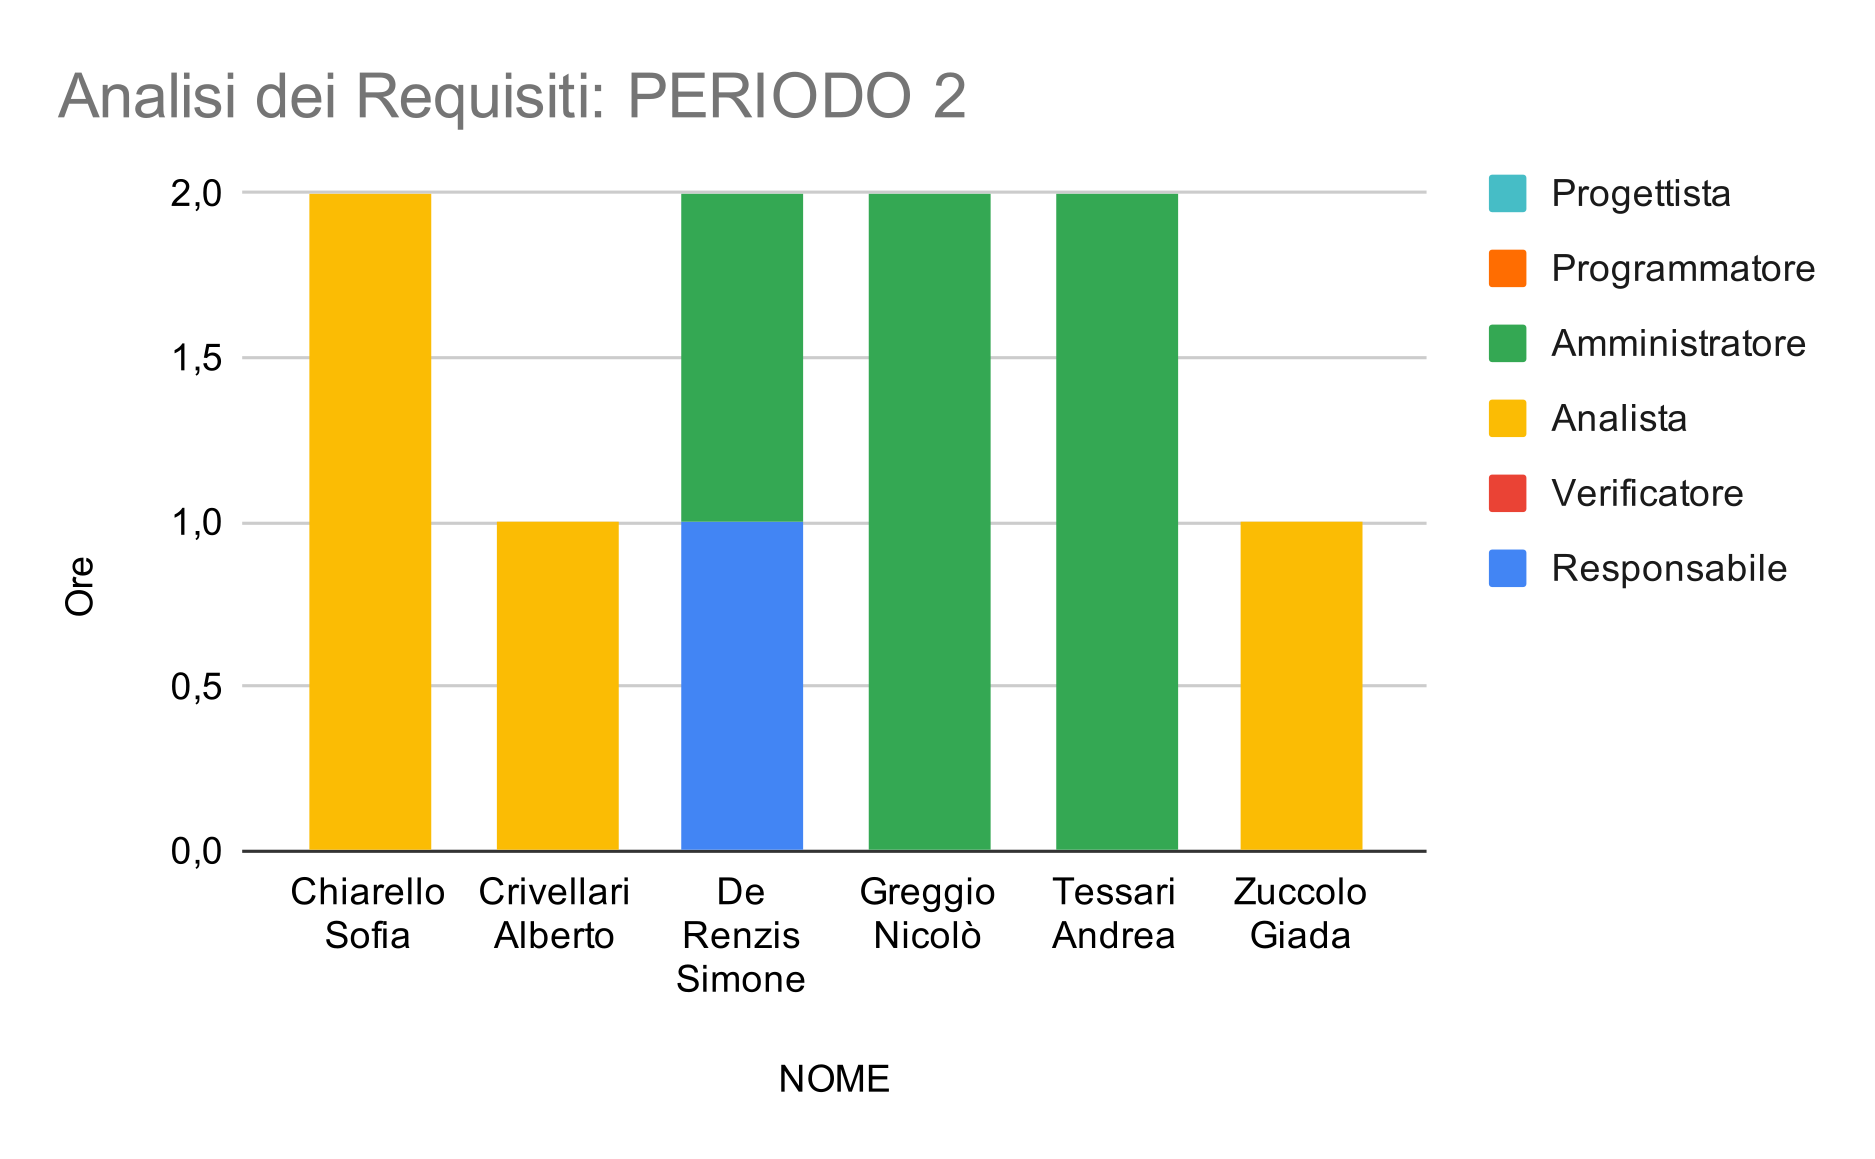
\includegraphics[scale=2]{res/images/charts/preventivo/analisi_2.png}
	\caption{Distribuzione oraria per componente: preventivo di periodo\textsubscript{G} - Analisi dei Requisiti - Periodo 2}
\end{figure}



\subsubsection{Riscontro di fine periodo}


\paragraph{Consuntivo orario ed economico}
\subparagraph*{}

\contabilitaTable{
	Chiarello Sofia & 0 & 0 & 1 & 0 & 0 & 0 & \textbf{1} \\ 
Crivellari Alberto & 0 & 1 & 0 & 0 & 0 & 0 & \textbf{1} \\ 
De Renzis Simone & 2 & 0 & 0 & 1 & 0 & 0 & \textbf{3} \\ 
Greggio Nicolò & 1 & 0 & 0 & 3 & 0 & 0 & \textbf{4} \\ 
Tessari Andrea & 0 & 0 & 0 & 1 & 0 & 0 & \textbf{1} \\ 
Zuccolo Giada & 0 & 0 & 1 & 0 & 0 & 0 & \textbf{1} \\ 
\hlinetable 
\textbf{Totale orario} & \textbf{3} & \textbf{1} & \textbf{2} & \textbf{5} & \textbf{0} & \textbf{0} & \textbf{11} \\ 
\textbf{Differenza orario} & \textbf{2} & \textbf{1} & \textbf{-2} & \textbf{0} & \textbf{0} & \textbf{0} & \textbf{1} \\ 
\textbf{Totale costi} & \textbf{90} & \textbf{15} & \textbf{50} & \textbf{100} & \textbf{0} & \textbf{0} & \textbf{255} \\ 
\textbf{Differenza costi} & \textbf{60} & \textbf{15} & \textbf{-50} & \textbf{0} & \textbf{0} & \textbf{0} & \textbf{25} \\ 
\end{tabular} 
\caption{Consuntivo - Analisi dei Requisiti - Periodo 2}
}

\begin{figure}[H]
	\centering
	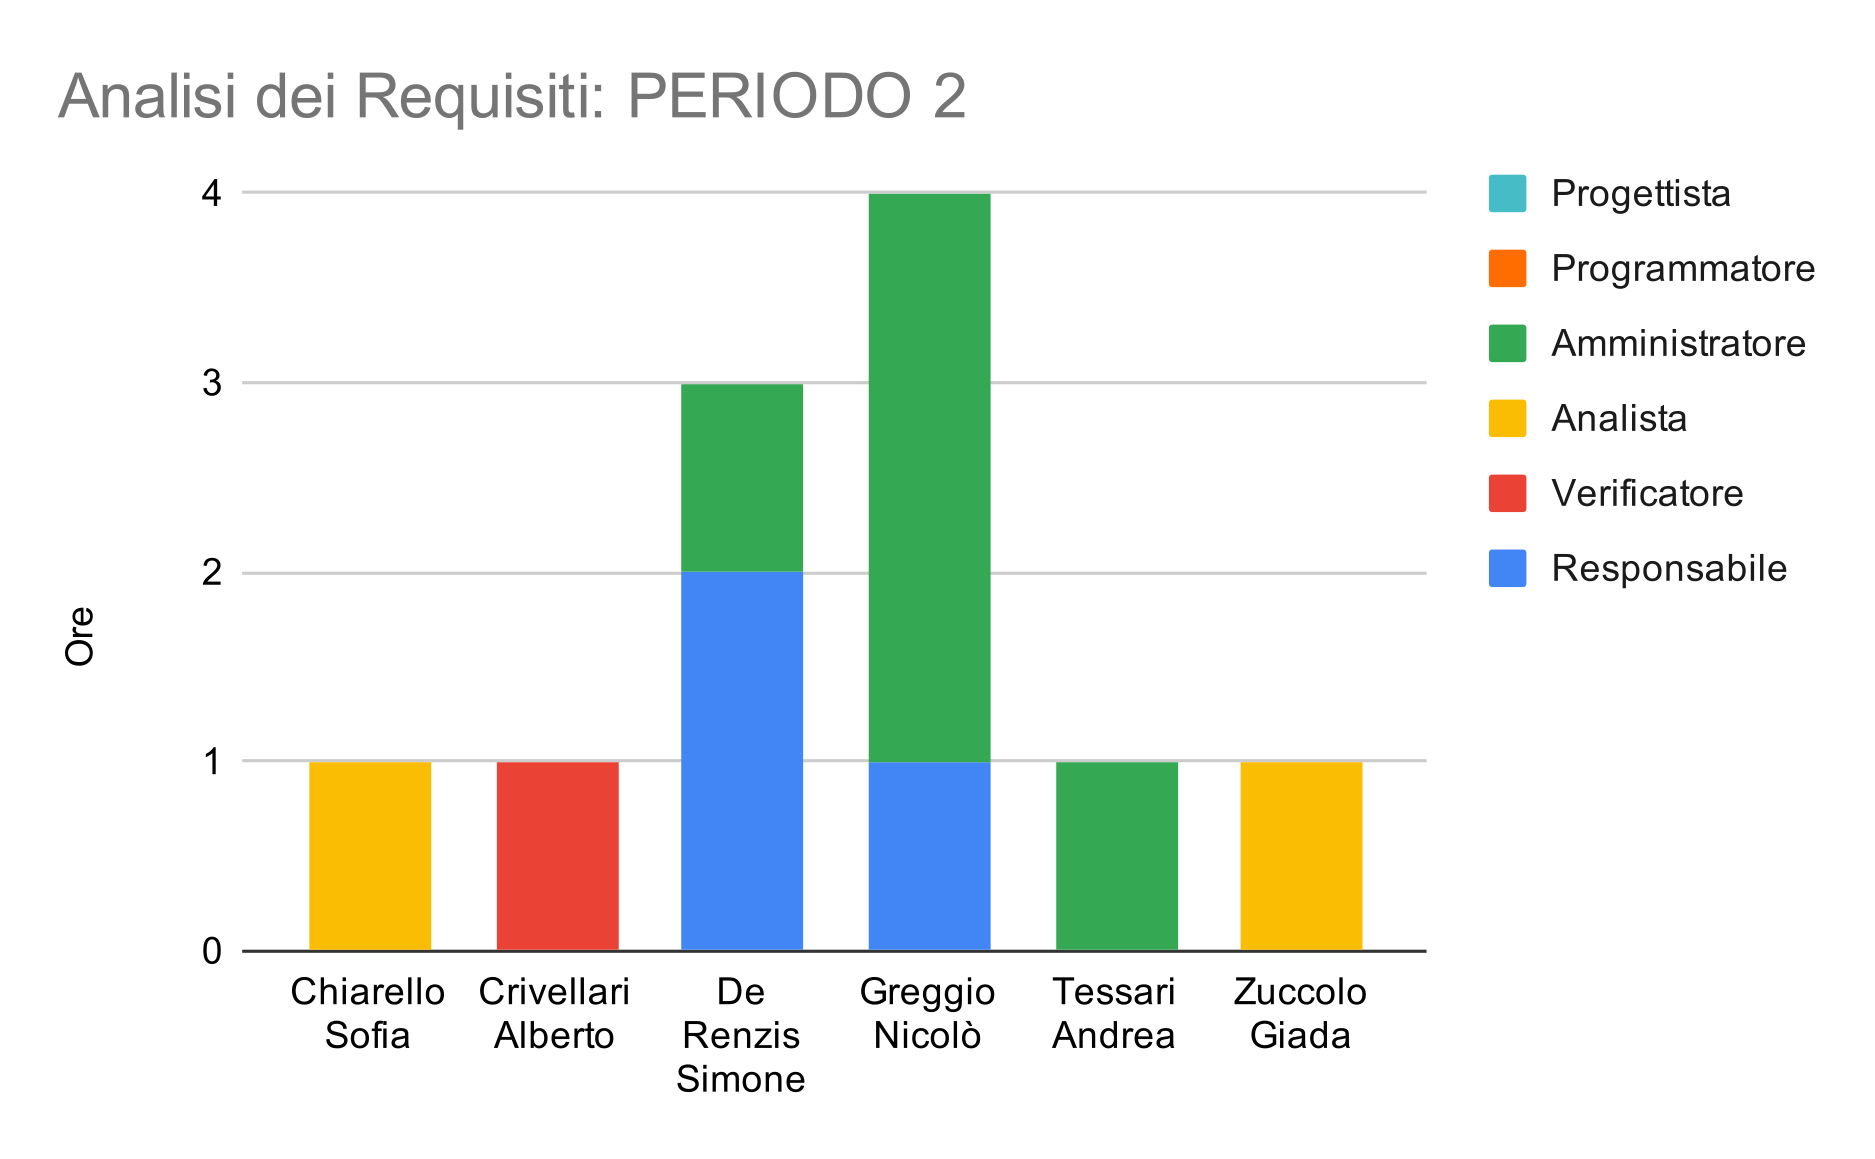
\includegraphics[scale=2]{res/images/charts/consuntivo/analisi_2.png}
	\caption{Distribuzione oraria per componente: consuntivo - Analisi dei Requisiti - Periodo 2}
\end{figure}

Il periodo\textsubscript{G} chiude in \textbf{negativo}, costringendo il gruppo ad una spesa supplementare di \textbf{25 \euro}. 


\paragraph{Preventivo a finire}
\subparagraph*{}

\pafTable{
	Avvio & 1 & Consuntivo & 
\tabularnewline
Analisi dei Requisiti & 1 & Consuntivo & 
\tabularnewline
Analisi dei Requisiti & 2 & Consuntivo & 
\tabularnewline
Progettazione Architetturale & 1 & Preventivo di periodo & 
\tabularnewline
Progettazione Architetturale & 2 & Preventivo & 2414
\tabularnewline
Progettazione Architetturale & 3 & Preventivo & 280
\tabularnewline
Progettazione di Dettaglio e Codifica & 1 & Preventivo & 1270
\tabularnewline
Progettazione di Dettaglio e Codifica & 2 & Preventivo & 4097
\tabularnewline
Progettazione di Dettaglio e Codifica & 3 & Preventivo & 258
\tabularnewline
Validazione e Collaudo & 1 & Preventivo & 220
\tabularnewline
Validazione e Collaudo & 2 & Preventivo & 2145
\tabularnewline
Validazione e Collaudo & 3 & Preventivo & 60
\tabularnewline
\textbf{Totale} & \textbf{} & \textbf{} & \textbf{10744}
\tabularnewline
\textbf{Totale rendicontato} & \textbf{} & \textbf{} & \textbf{10744}
\tabularnewline
\caption{Preventivo a finire - Analisi dei Requisiti - Periodo 2}
}